\documentclass{beamer}
\usepackage[utf8]{inputenc} % allow utf-8 input
\usepackage[T1]{fontenc}    % use 8-bit T1 fonts
\usepackage{hyperref}       % hyperlinks
\usepackage{url}            % simple URL typesetting
\usepackage{booktabs}       % professional-quality tables
\usepackage{amsfonts}       % blackboard math symbols
\usepackage{nicefrac}       % compact symbols for 1/2, etc.
\usepackage{microtype}      % microtypography
\usepackage{amsmath}
\usepackage{tikz}
\usetikzlibrary{calc}
\usetikzlibrary{bayesnet}
\usetikzlibrary{arrows}
\usepackage{color}
\usepackage{array}
\usepackage{dsfont}
\usepackage{multirow, graphicx}
 \usepackage{float}
\newcolumntype{C}[1]{>{\centering\arraybackslash}p{#1}}
\newcolumntype{R}[1]{>{\raggedleft\arraybackslash}p{#1}}
\newcolumntype{L}[1]{>{\raggedright\arraybackslash}p{#1}}
\usepackage{caption}
\usepackage{subfig}
\usepackage{pifont}
\usepackage{xcolor}
\usepackage{algorithm,algorithmic}
\newcommand{\cmark}{\textcolor{green!80!black}{\ding{51}}}
\newcommand{\xmark}{\textcolor{red}{\ding{55}}}
\DeclareMathOperator*{\argmin}{argmin}
\urlstyle{same}
\usepackage{listings}
% \usetheme{Boadilla}

\title{Introduction to Differentiable Probabilistic Models}
% \subtitle{Using Beamer}
\author{Bill Watson}
\institute{S\&P Global}
\date{\today}

\begin{document}

\begin{frame}
\titlepage
\end{frame}


\begin{frame}
\frametitle{Primer: Standard Machine Learning}
\begin{itemize}
\item Usually, we are given a set $\mathcal{D} = \{ X, y\}$
  \begin{equation*}
  X =
    \begin{bmatrix}
        x_{11} & x_{12} & \dots  & x_{1m} \\
        x_{21} & x_{22} & \dots  & x_{2m} \\
        \vdots & \vdots & \ddots & \vdots \\
        x_{n1} & x_{n2} & \dots  & x_{nm}
    \end{bmatrix}
    \quad \quad
    y =
    \begin{bmatrix}
      y_1 \\
      y_2 \\
      \vdots \\
      y_n
    \end{bmatrix}
  \end{equation*}
  where $X$ is our data matrix, and $y$ are our labels.
\pause
\item Attempt to fit a model $f$ parameterized by $\theta$ with respect to
an objective function $\mathcal{L}$
\begin{equation*}
  \theta^{*}  =  \argmin_{\theta} \; \mathcal{L} \big( f( X;\theta), \; y \big)
\end{equation*}
\end{itemize}
\end{frame}


\begin{frame}
\frametitle{Reframed as a Probabilistic Model}
\begin{itemize}
\item Consider our model is a probability distribution $Q$
\begin{itemize}
  \item No longer have labels $y$
  \item But have probabilities and sampling
\end{itemize}
\pause
\item Consider that our data is sampled from the real world $P$:
\begin{equation*}
  \begin{gathered}
  X \sim P \\
  \theta^{*} = \argmin_{\theta} \; \mathcal{L} \big( f(X;\theta) \big) \\
\end{gathered}
\end{equation*}
\pause
\item Examples:
\begin{itemize}
  \item Classification: Fitting two multinomial distributions
  \item Regression: Fitting a Normal centered around the line of best fit
\end{itemize}
\end{itemize}
\end{frame}

\begin{frame}
  \frametitle{How do we "fit" Distributions?}
  \begin{itemize}
    \item Fitting two distributions implies minimizing their difference,
      i.e. "distance"
    \item This "distance" is known as the divergence between the true distribution
    $P$ and the learned distribution Q.
    \pause
    \item Divergences must satisfy 2 properties:
    \begin{itemize}
      \item $D(P \parallel Q ) \geq 0 \quad \forall P, Q \in S$
      \item $D(P \parallel Q ) = 0 \iff P = Q$
    \end{itemize}
  \end{itemize}

\end{frame}

\begin{frame}
  \frametitle{The Kullback-Leibler Divergence}
  \begin{itemize}
    \item The KL Divergence for distributions $P$ and $Q$ is defined as:
    \begin{equation*}
      D_{KL} (P \parallel Q) = \int_{-\infty}^{\infty} p(x)\log \left({\frac {p(x)}{q(x)}}\right)\,dx
    \end{equation*}
    \pause
    \item Note: the KL Divergence is NOT symmetric:
    \begin{equation*}
      D_{KL} (P \parallel Q) \not= D_{KL} (Q \parallel P)
    \end{equation*}
    \item Hence, this direction is known as the Forward KL
    \pause
    \item But we will come back to this later...
  \end{itemize}
\end{frame}


\begin{frame}
  \frametitle{Digression: Monte Carlo Integration}
    \begin{equation*}
      \begin{aligned}
      D_{KL} (P \parallel Q) =& \int_{-\infty}^{\infty} p(x)\log \left({\frac {p(x)}{q(x)}}\right)\,dx \\
      \pause
      =& \; \mathbb{E}_{x \sim P} \left[ \log \left( \frac{p(x)}{q(x)} \right) \right] \\
      \pause
      \approx& \frac{1}{N}\sum_{i=1}^{N} \log \left( \frac{p(x_i)}{q(x_i)} \right) \quad x_i \sim P \vert_{i=1}^{N}
      \end{aligned}
    \end{equation*}
\end{frame}


\begin{frame}
  \frametitle{Digression: Monte Carlo Integration}
    \begin{equation*}
      \begin{aligned}
      D_{KL} (P \parallel Q) =& \int_{-\infty}^{\infty} p(x)\log \left({\frac {p(x)}{q(x)}}\right)\,dx \\
      =& \; \mathbb{E}_{x \sim P} \left[ \log \left( \frac{p(x)}{q(x)} \right) \right] \\
      \approx& \frac{1}{N}\sum_{i=1}^{N} \log \left( \frac{p(x_i)}{q(x_i)} \right) \quad x_i \sim P \vert_{i=1}^{N}
      \end{aligned}
    \end{equation*}
    \begin{algorithm}[H]
    \begin{algorithmic}[1]
      \STATE $x_1, \hdots, x_n \sim P$ independently
      \RETURN $\frac{1}{N}\sum_{x_i} f(x_i)$
    \end{algorithmic}
    \caption{$\mathbb{E}_{x \sim P}[f(x)]$\\Expectation of $f(x)$ with respect to $P$}
    \end{algorithm}
\end{frame}


\begin{frame}
  \frametitle{Digression: KL to Cross-Entropy}
  \begin{itemize}
    \item Note: Maximum Likelihood Estimation is equivalent to minimizing the Forward KL
    \pause
    \item The KL Divergence can be decomposed into familiar terms:
  \end{itemize}
  \begin{equation*}
    \begin{aligned}
      \argmin_{Q} D_{KL} (P \parallel Q) =& \argmin_{Q} \sum_{x \in \mathcal {X}} p(x)\log \left({\frac {p(x)}{q(x)}}\right) \\
      \pause
      =& \argmin_{Q} - \sum_{x \in \mathcal {X}} p(x)\log q(x) \\
      & \quad\quad\quad + \sum_{x \in \mathcal {X}} p(x)\log p(x) \\
      \pause
      =& \argmin_{Q} \underbrace{H(P, Q)}_{Cross-Entropy} - \underbrace{H(P)}_{Entropy} \\
      \pause
      =& \argmin_{Q} \underbrace{H(P, Q)}_{Cross-Entropy}
    \end{aligned}
  \end{equation*}
\end{frame}

\begin{frame}
  \frametitle{Digression: KL to Cross-Entropy}
  \begin{itemize}
    \item If we consider $P(y_i = 1 | x_i) = p_i$ and $Q(y_i = 1 | x_i) = \sigma(f_\theta (x_i))$:
  \end{itemize}
  \begin{equation*}
    \begin{aligned}
      \argmin_{\theta} \; & D_{KL} (P \parallel Q) = \\
        & \argmin_{\theta} - \Big[ p_i \log \sigma\big(f_\theta (x_i)\big) + (1 - p_i) \log (1 - \sigma \big(f_\theta (x_i))\big) \Big]
    \end{aligned}
  \end{equation*}
  \begin{itemize}
    \item This is the Binary Cross-Entropy Loss
  \end{itemize}
\end{frame}


\begin{frame}
  \frametitle{Forward KL: Learning a Normal Distribution (Initial)}
  \begin{figure}
    \centering
    \includegraphics[scale=0.6]{assets/forward_kl_normal_init}
    \caption{$P \sim \mathcal{N}(-7.3, 3.2)$, $Q \sim \mathcal{N}(0, 1)$}
  \end{figure}
\end{frame}

\begin{frame}
  \frametitle{Forward KL: Learning a Normal Distribution (Results)}
  \begin{figure}
    \centering
    \includegraphics[height=4.3cm]{assets/forward_kl_normal_stats}
  \end{figure}
  \begin{figure}
    \centering
    \includegraphics[height=2.5cm]{assets/forward_kl_normal_result}
    \caption{$P \sim \mathcal{N}(-7.3, 3.2)$, $Q \sim \mathcal{N}(-7.28, 3.24)$}
  \end{figure}
\end{frame}


\begin{frame}
  \frametitle{Digression: Gaussian Mixture Models}
  \begin{itemize}
    \item We can build a $K$ multi-modal distribution, with weights
      $\mathbf{\pi}$, as follows:
    \begin{equation*}
      \begin{aligned}
      z \; \sim& \; \text{Categorical}(\mathbf{\pi}) \\
      x \,|\, z = k \; \sim& \; \text{Normal}(\mu_k, \sigma_k) \\
    \end{aligned}
    \end{equation*}
    \item We can calculate log probabilities by marginalizing out $z$:
    \begin{equation*}
      \log p(x) = \log \sum_{k=1}^{K} \underbrace{p(z = k)}_{\text{Categorical}} \cdot \underbrace{p(x \,|\, z=k)}_{\text{Normal}}
    \end{equation*}
  \end{itemize}
\end{frame}

\begin{frame}
  \frametitle{Digression: Mixture Models (Visual)}
  \begin{columns}
    \centering
    \begin{column}{0.48\textwidth}
      \begin{figure}
        \centering
        \includegraphics[scale=0.4]{assets/bimodal_example_1}
        \caption{2 Mixture Components, Even Weights}
      \end{figure}
    \end{column}
    \begin{column}{0.48\textwidth}
      \begin{figure}
        \centering
        \includegraphics[scale=0.4]{assets/bimodal_example_2}
        \caption{3 Mixture Components, Uneven Weights}
      \end{figure}
    \end{column}
  \end{columns}
\end{frame}


\begin{frame}
  \frametitle{Forward KL: Learning a Bimodal (Initial)}
  \begin{figure}
    \centering
    \includegraphics[scale=0.6]{assets/forward_kl_bimodal_init}
    \caption{$P \sim \big\{\mathcal{N}(-7.3, 1.4), \; \mathcal{N}(7.3, 1.4) \big\}$\\$Q \sim \mathcal{N}(0, 1)$}
  \end{figure}
\end{frame}


\begin{frame}
  \frametitle{Forward KL: Learning a Bimodal (Results)}
  \begin{figure}
    \centering
    \includegraphics[height=2.5cm]{assets/forward_kl_bimodal_stats}
  \end{figure}
  \begin{figure}
    \centering
    \includegraphics[height=4.3cm]{assets/forward_kl_bimodal_result}
    \caption{$Q \sim \mathcal{N}(0.08, 36.76)$}
  \end{figure}
\end{frame}

\begin{frame}
  \frametitle{Forward KL: Zero-Avoiding}
  \begin{equation*}
    D_{KL} (P \parallel Q) = \int_{-\infty}^{\infty} \overbrace{p(x)}^{\text{Constant}}\log \left({\frac {\overbrace{p(x)}^{\text{Constant}}}{\underbrace{q(x)}_{Variable}}}\right)\,dx
  \end{equation*}
  \begin{itemize}
    \item $p(x)$ is constant-valued, $q(x)$ is variable
    \item If $Q$ does not support $P$, then we will sample a point that has a low
      probability with respect to $Q$
    \pause
    \item As $q(x) \to 0$, our loss $D_{KL} \to \infty$
    \pause
    \item Hence, the optimal solution is for $Q$ to cover $P$, i.e. averaging
  \end{itemize}
\end{frame}

\begin{frame}
  \frametitle{Forward KL: Loss Landscape}
  \begin{figure}
    \centering
    \includegraphics[scale=0.6]{assets/forward_kl_bimodal_loss}
    \caption{Loss Landscape for Forward KL Divergence}
  \end{figure}
\end{frame}


\begin{frame}
  \frametitle{Directionality: Reverse KL}
  \begin{equation*}
    \begin{aligned}
    D_{KL} (Q \parallel P) =& \int_{-\infty}^{\infty} q(x)\log \left({\frac {q(x)}{p(x)}}\right)\,dx \\
    =& \; \mathbb{E}_{x \sim Q} \left[ \log \left( \frac{q(x)}{p(x)} \right) \right]
    \end{aligned}
  \end{equation*}
  \begin{itemize}
    \item The Reverse KL will sample from $Q$, and evaluate the log probabilities from $P$ and $Q$
    \item Recall: KL Divergence is not symmetric, and this has drastic implications...
  \end{itemize}
\end{frame}


\begin{frame}
  \frametitle{Digression: Differentiable Sampling via the Reparameterization Trick}
  \begin{figure}
    \centering
    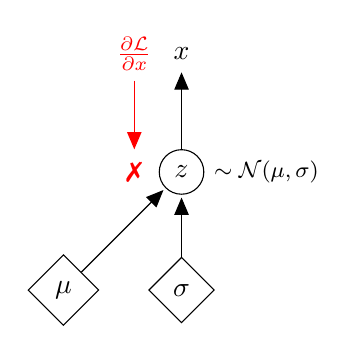
\begin{tikzpicture}[shorten >=1pt,node distance=1.5cm,on grid,auto]
      \node[draw,diamond]  (sig)  {$\sigma$};
      \node[draw,diamond]  (mu)  [left=of sig] {$\mu$};
      \node[draw,circle]   (z) [above=of sig, label=right:{$\sim \mathcal{N}(\mu, \sigma)$}] {$z$};
      \node[] (x) [above=of z] {$x$};
      \node[red] (l1) [left=of x, xshift=0.9cm] {$\frac{\partial \mathcal{L}}{\partial x}$};
      \node[red] (l2) [left=of z, xshift=0.9cm] {\xmark};
      \draw[->] (sig) to (z) node [] {};
      \draw[->] (mu) to (z) node [] {};
      \draw[->] (z) to (x) node [] {};
      \draw[red,->] (l1) to (l2) node [] {};
    \end{tikzpicture}
    \caption{Original Form}
  \end{figure}
\end{frame}


\begin{frame}
  \frametitle{Digression: Differentiable Sampling via the Reparameterization Trick}
    \begin{figure}
      \centering
      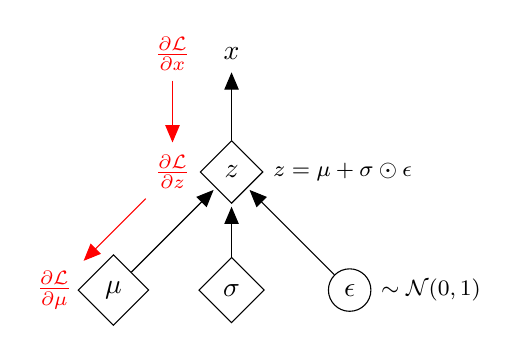
\begin{tikzpicture}[shorten >=1pt,node distance=1.5cm,on grid,auto]
        \node[draw,diamond]  (sig)  {$\sigma$};
        \node[draw,diamond]  (mu)  [left=of sig] {$\mu$};
        \node[draw,diamond]  (z) [above=of sig, label=right:{$z = \mu + \sigma \odot \epsilon$}] {$z$};
        \node[draw,circle]   (e) [right=of sig, label=right:{$\sim \mathcal{N}(0, 1)$}] {$\epsilon$};
        \node[] (x) [above=of z] {$x$};
        \node[red] (l1) [left=of x, xshift=0.75cm] {$\frac{\partial \mathcal{L}}{\partial x}$};
        \node[red] (l2) [left=of z, xshift=0.75cm] {$\frac{\partial \mathcal{L}}{\partial z}$};
        \node[red] (l3) [left=of mu, xshift=0.75cm] {$\frac{\partial \mathcal{L}}{\partial \mu}$};
        \draw[->] (sig) to (z);
        \draw[->] (mu) to (z);
        \draw[->] (e) to (z);
        \draw[->] (z) to (x);
        \draw[red,->] (l1) to (l2);
        \draw[red,->] (l2) to (l3);
      \end{tikzpicture}
      \caption{Reparameterized Version}
    \end{figure}
\end{frame}



\begin{frame}
  \frametitle{Digression: Common Reparameterization Tricks}
  \begin{center}
  \begin{tabular}{C{5cm}C{5cm}}
  \toprule
  {} & Reparameterized \\
  \midrule
  $\mathcal{N}(\mu, \sigma)$   &  $\mu + \sigma \cdot \mathcal{N}(0, 1)$ \\
  \\
  $\text{Uniform}(a, b)$   &  $a + (b - a) \cdot \mathcal{U}(0, 1)$ \\
  \\
  $\text{Exp}(\lambda)$   &  $\text{Exp}(1) / \lambda$ \\
  \\
  $\text{Cauchy}(\mu, \gamma)$   &  $\mu + \gamma \cdot \text{Cauchy}(0, 1)$ \\
  \bottomrule
  \end{tabular}
  \end{center}
\end{frame}

\begin{frame}
  \frametitle{Digression: Common Reparameterization Tricks}
  \begin{center}
  \begin{tabular}{C{5cm}C{5cm}}
  \toprule
  {} & Reparameterized \\
  \midrule
  $\mathcal{N}(\mu, \sigma)$   &  $\mu + \sigma \cdot \mathcal{N}(0, 1)$ \\
  \\
  $\mathcal{U}(a, b)$   &  $a + (b - a) \cdot \mathcal{U}(0, 1)$ \\
  \\
  $\text{Exp}(\lambda)$   &  $\text{Exp}(1) / \lambda$ \\
  \\
  $\text{Cauchy}(\mu, \gamma)$   &  $\mu + \gamma \cdot \text{Cauchy}(0, 1)$ \\
  \\
  \multirow{2}{*}{$\text{Laplace}(\mu, b)$}  &  $u \sim \text{Uniform}(-1, 1)$ \\
                                          & $\mu - b \cdot \text{sgn}(u) \ln \big[ 1 - \vert u \vert \big]$ \\
  \bottomrule
  \end{tabular}
  \end{center}
\end{frame}

\begin{frame}
  \frametitle{Digression: Common Reparameterization Tricks}
  \begin{center}
  \begin{tabular}{C{5cm}C{5cm}}
  \toprule
  {} & Reparameterized \\
  \midrule
  $\mathcal{N}(\mu, \sigma)$   &  $\mu + \sigma \cdot \mathcal{N}(0, 1)$ \\
  \\
  $\text{Uniform}(a, b)$   &  $a + (b - a) \cdot \mathcal{U}(0, 1)$ \\
  \\
  $\text{Exp}(\lambda)$   &  $\text{Exp}(1) / \lambda$ \\
  \\
  $\text{Cauchy}(\mu, \gamma)$   &  $\mu + \gamma \cdot \text{Cauchy}(0, 1)$ \\
  \\
  \multirow{2}{*}{$\text{Laplace}(\mu, b)$}  &  $u \sim \text{Uniform}(-1, 1)$ \\
                                          & $\mu - b \cdot \text{sgn}(u) \ln \big[ 1 - \vert u \vert \big]$ \\
                                          \\
  $\text{Categorical}(\pi)$ & \xmark \\
  \bottomrule
  \end{tabular}
  \end{center}
\end{frame}

\begin{frame}
  \frametitle{Reverse KL: Learning a Bimodal (Initial)}
  \begin{figure}
    \centering
    \includegraphics[scale=0.6]{assets/reverse_kl_bimodal_init}
    \caption{$P \sim \big\{\mathcal{N}(-7.3, 1.4), \; \mathcal{N}(7.3, 1.4) \big\}$\\$Q \sim \mathcal{N}(0, 1)$}
  \end{figure}
\end{frame}

\begin{frame}
  \frametitle{Reverse KL: Learning a Bimodal (Results)}
  \begin{figure}
    \centering
    \includegraphics[height=2.5cm]{assets/reverse_kl_bimodal_stats_1}
  \end{figure}
  \begin{figure}
    \centering
    \includegraphics[height=4.3cm]{assets/reverse_kl_bimodal_result_1}
    \caption{$Q \sim \mathcal{N}(-7.02, 1.41)$}
  \end{figure}
\end{frame}


\begin{frame}
  \frametitle{Reverse KL: Learning a Bimodal Attempt 2 (Results)}
  \begin{figure}
    \centering
    \includegraphics[height=2.5cm]{assets/reverse_kl_bimodal_stats_2}
  \end{figure}
  \begin{figure}
    \centering
    \includegraphics[height=4.3cm]{assets/reverse_kl_bimodal_result_2}
    \caption{$Q \sim \mathcal{N}(7.01, 1.46)$}
  \end{figure}
\end{frame}


\begin{frame}
  \frametitle{Reverse KL: Zero-Forcing}
  \begin{equation*}
    D_{KL} (Q \parallel P) = \int_{-\infty}^{\infty} q(x)\log \left({\frac {q(x)}{p(x)}}\right)\,dx
  \end{equation*}
  \begin{columns}
    \begin{column}{0.48\textwidth}
    \begin{itemize}
      \item Unlike the Forward KL, Reverse KL is Zero-forcing
      \item Why? Because we no longer suffer a penalty from $q(x) = 0$
      \item However, if $p(x) = 0$, then the optimal value for $q(x)$ is $0$
      \item Result $\implies$ Mode Collapse
    \end{itemize}
    \end{column}
    \begin{column}{0.48\textwidth}
      \begin{figure}
        \centering
        \includegraphics[scale=0.4]{assets/reverse_kl_bimodal_loss}
        \caption{Loss Landscape for Reverse KL Divergence}
      \end{figure}
    \end{column}
  \end{columns}
\end{frame}


\begin{frame}
  \frametitle{Jensen - Shannon Divergence: A Symmetric Divergence}
  \begin{equation*}
    \begin{aligned}
      \text{JSD}(P \parallel Q) \;=&\; \frac{1}{2} D_{KL}(P \parallel M) + \frac{1}{2} D_{KL}(Q \parallel M) \\
      M \;=&\; \frac{1}{2} (P + Q)
    \end{aligned}
  \end{equation*}
  \begin{itemize}
    \item The JS Divergence is a symmetrized version of the
      KL Divergence
    \item $M$ is the average of distributions $P$ and $Q$, and can be
      represented as a Mixture Model
  \end{itemize}
\end{frame}


\begin{frame}
  \frametitle{Jensen - Shannon Divergence: Bimodal (Initial)}
  \begin{figure}
    \centering
    \includegraphics[scale=0.6]{assets/js_bimodal_center_init}
    \caption{$P \sim \big\{\mathcal{N}(-7.3, 1.4), \; \mathcal{N}(7.3, 1.4) \big\}$\\$Q \sim \mathcal{N}(0, 1)$}
  \end{figure}
\end{frame}

\begin{frame}
  \frametitle{Jensen - Shannon Divergence: Bimodal (Result)}
  \begin{figure}
    \centering
    \includegraphics[height=2.5cm]{assets/js_bimodal_center_stats}
  \end{figure}
  \begin{figure}
    \centering
    \includegraphics[height=4.3cm]{assets/js_bimodal_center_result}
    \caption{$Q \sim \mathcal{N}(-0.04, 48.20)$}
  \end{figure}
\end{frame}


\begin{frame}
  \frametitle{Jensen - Shannon Divergence: Right Shift (Attempt 2)}
  \begin{figure}
    \centering
    \includegraphics[scale=0.6]{assets/js_bimodal_right_init}
    \caption{$P \sim \big\{\mathcal{N}(-7.3, 1.4), \; \mathcal{N}(7.3, 1.4) \big\}$\\$Q \sim \mathcal{N}(1, 1)$}
  \end{figure}
\end{frame}

\begin{frame}
  \frametitle{Jensen - Shannon Divergence: Right Shift (Result)}
  \begin{figure}
    \centering
    \includegraphics[height=2.5cm]{assets/js_bimodal_right_stats}
  \end{figure}
  \begin{figure}
    \centering
    \includegraphics[height=4.3cm]{assets/js_bimodal_right_result}
    \caption{$Q \sim \mathcal{N}(6.99, 1.43)$}
  \end{figure}
\end{frame}


\begin{frame}
  \frametitle{Jensen - Shannon Divergence: Left Shift (Attempt 3)}
  \begin{figure}
    \centering
    \includegraphics[scale=0.6]{assets/js_bimodal_left_init}
    \caption{$P \sim \big\{\mathcal{N}(-7.3, 1.4), \; \mathcal{N}(7.3, 1.4) \big\}$\\$Q \sim \mathcal{N}(-1, 1)$}
  \end{figure}
\end{frame}

\begin{frame}
  \frametitle{Jensen - Shannon Divergence: Left Shift (Result)}
  \begin{figure}
    \centering
    \includegraphics[height=2.5cm]{assets/js_bimodal_left_stats}
  \end{figure}
  \begin{figure}
    \centering
    \includegraphics[height=4.3cm]{assets/js_bimodal_left_result}
    \caption{$Q \sim \mathcal{N}(-6.98, 1.38)$}
  \end{figure}
\end{frame}

\begin{frame}
  \frametitle{Jensen - Shannon Divergence Loss}
  \begin{equation*}
    \begin{aligned}
      \text{JSD}(P \parallel Q) \;=&\; \frac{1}{2} D_{KL}(P \parallel M) + \frac{1}{2} D_{KL}(Q \parallel M) \\
      M \;=&\; \frac{1}{2} (P + Q)
    \end{aligned}
  \end{equation*}
  \begin{figure}
    \centering
    \includegraphics[scale=0.5]{assets/js_bimodal_loss}
    \caption{Loss Landscape for JS Divergence}
  \end{figure}
\end{frame}


\begin{frame}
  \frametitle{A Family of Divergences: $f$-Divergence}
  \begin{itemize}
    \item KL Divergence is a special case of the $f$-divergence
    \item The $f$-divergence is a family of divergences that can be written as:
    \begin{equation*}
      D_{f}(P \parallel Q) = \int \overbrace{q(x)}^{\text{Weight}} f \underbrace{\left( \frac{p(x)}{q(x)} \right)}_{\text{Odds Ratio}} dx
    \end{equation*}
  \end{itemize}
\end{frame}

\begin{frame}
  \frametitle{A Family of Divergences: $f$-Divergence}
  \begin{equation*}
    D_{f}(P \parallel Q) = \int \overbrace{q(x)}^{\text{Weight}} f \underbrace{\left( \frac{p(x)}{q(x)} \right)}_{\text{Odds Ratio}} dx
  \end{equation*}
  \begin{center}
  \begin{tabular}{C{5cm}|C{5cm}}
  \toprule
  {Divergence} & $f(t)$ \\
  \midrule
  Forward KL   &  $t \log t$ \\
  Reverse KL   &  $- \log t$ \\
  Hellinger Distance  &  $\left(\sqrt{t} - 1 \right)^2$, $2 \left( 1 - \sqrt{t} \right)$ \\
  Total Variation & $\frac{1}{2} \vert t - 1 \vert$ \\
  Pearson $\chi^2$ & $\left( t-1 \right)^2$, $t^2 - 1$, $t^2 - t$ \\
  Neyman $\chi^2$ (Reverse Pearson) & $\frac{1}{t} - 1$, $\frac{1}{t} - t$ \\
  \bottomrule
  \end{tabular}
  \end{center}
\end{frame}


\begin{frame}
  \frametitle{Earth Mover's Distance (Wasserstein Distance)}
  \begin{equation*}
    \text{EMD}\left(P_r, P_{\theta}\right) = \inf_{\gamma \in \prod} \sum_{x, y} \overbrace{\parallel x - y \parallel}^{\ell_2 \text{Norm}} \underbrace{\gamma \left( x, y \right)}_{\text{Joint Marginal}}
  \end{equation*}
  \begin{itemize}
    \item For discrete distributions $P_r$, $P_{\theta}$
    \item $\gamma \left( x, y \right)$ states how we distribute the amount of "earth" from one place $x$ over the domain of $y$, or vice versa
    \item EMD is the minimal total amount of work it takes to transform one distribution into the other
  \end{itemize}
  \begin{columns}
    \begin{column}{0.48\textwidth}
      \begin{figure}
        \centering
        \includegraphics[width=5cm]{assets/emd_hist_1}
      \end{figure}
    \end{column}
    \begin{column}{0.48\textwidth}
      \begin{figure}
        \centering
        \includegraphics[width=5cm]{assets/emd_hist_2}
      \end{figure}
    \end{column}
  \end{columns}
\end{frame}

\begin{frame}
  \frametitle{Earth Mover's Distance (Wasserstein Distance)}
  \begin{equation*}
    \text{EMD}\left(P_r, P_{\theta}\right) = \inf_{\gamma \in \prod} \sum_{x, y} \parallel x - y \parallel  \gamma \left( x, y \right)
  \end{equation*}
  \begin{figure}
    \centering
    \includegraphics[height=3.75cm]{assets/transport_plan}
  \end{figure}
  \begin{figure}
    \centering
    \includegraphics[height=2.2cm]{assets/earth_move}
  \end{figure}
\end{frame}


\begin{frame}
  \frametitle{Summary of Methods}
  \begin{center}
  \begin{tabular}{lC{1.5cm}|C{1.5cm}|C{1.5cm}|C{1.5cm}}
  \toprule
  {} & \multicolumn{2}{c}{$P$} & \multicolumn{2}{c}{$Q$} \\
  \cmidrule(lr){2-3}  \cmidrule(lr){4-5}
  {} &  \multicolumn{1}{c}{$\log p(x)$} &  \multicolumn{1}{c|}{$x \sim P$} &  \multicolumn{1}{c}{$\log q(x)$} &  \multicolumn{1}{c}{$x \sim Q$} \\
  \midrule
  Cross-Entropy    &        & \cmark & \cmark &        \\
  Forward KL       & \cmark & \cmark & \cmark &        \\
  Reverse KL       & \cmark &        & \cmark & \cmark \\
  JS Divergence    & \cmark & \cmark & \cmark & \cmark \\
  $f$-Divergence   & \cmark & \cmark & \cmark & \cmark \\
  \bottomrule
  \end{tabular}
  \end{center}
\end{frame}


\begin{frame}
  \frametitle{Practical Uses of Divergences}
  \begin{itemize}
    \item Forward Kullback-Leibler
    \begin{itemize}
      \item Maximum Likelihood Estimation
      \begin{itemize}
        \item $\ell_2$: Mean Squared Error (Normally Distributed)
        \item $\ell_1$: Mean Absolute Error (Laplace Distributed)
        \item Binary Cross Entropy (Bernoulli Distributed)
        \item Cross Entropy (Multinomially Distributed)
      \end{itemize}
      \item Log-Likelihood Models
      \begin{itemize}
        \item PixelCNN
        \item Glow
        \item Variational Autoencoders
      \end{itemize}
    \end{itemize}
  \end{itemize}
\end{frame}


\begin{frame}
  \frametitle{Practical Uses of Divergences}
  \begin{itemize}
    \item Reverse Kullback-Leibler
      \begin{itemize}
        \item Evidence Lower Bound (ELBO)
      \end{itemize}
    \item Jensen-Shannon Divergence
      \begin{itemize}
        \item Generative Adversarial Network (Original)
      \end{itemize}
    \item Earth Mover's Distance
      \begin{itemize}
        \item Wasserstein GAN (WGAN)
      \end{itemize}
    \item Pearson $\chi^2$ Divergence
      \begin{itemize}
        \item Least Squares GAN (LSGAN)
      \end{itemize}
  \end{itemize}
\end{frame}


\begin{frame}
  \frametitle{Potpourri: Advanced Techniques}
  \begin{enumerate}
    \item Transforms
      \begin{itemize}
        \item Normalizing Flow Models
      \end{itemize}
    \item Expectation–Maximization
    \item Variational Inference
      \begin{itemize}
        \item ELBO
      \end{itemize}
    \item Adversarial Training (GANs, GANs, GANs)
    \item Markov Chain Monte Carlo
    \begin{itemize}
      \item Metropolis-Hastings
      \item Gibbs Sampling
      \item Hamiltonian Monte Carlo
      \item NUTS
    \end{itemize}
  \end{enumerate}
\end{frame}


\end{document}
